% OmniMed-FL --- controlled-v3 real-radiograph submission source.
% Every quantitative claim and result figure is sourced from the frozen v3
% store and its provenance-checked merged artifact.
\documentclass[letterpaper, conference]{IEEEtran}
\IEEEoverridecommandlockouts

% Strict margin enforcement and text wrapping
\usepackage[letterpaper, top=0.75in, bottom=1in, left=0.625in, right=0.625in]{geometry}
\usepackage{microtype}

\usepackage{cite}
\usepackage{amsmath,amssymb,amsfonts}
\usepackage{graphicx}
\usepackage{textcomp}
\usepackage{xcolor}
\usepackage{booktabs}
\usepackage{url}
\usepackage{placeins}
\usepackage{balance}
% \usepackage{stfloats}  % not installed in all TeX distributions; no [b] figure* is used
\usepackage{tikz}
\usetikzlibrary{arrows.meta,shapes.geometric,positioning,fit,backgrounds,calc}

\definecolor{llmblue}   {RGB}{76,114,176}
\definecolor{vitgreen}  {RGB}{85,168,104}
\definecolor{vlmred}    {RGB}{196,78,82}
\definecolor{fedorange} {RGB}{204,185,116}
\definecolor{fedpurple} {RGB}{129,114,178}
\definecolor{outyyellow}{RGB}{255,242,204}
\definecolor{smallgray} {RGB}{220,220,220}
\definecolor{fignavy}   {RGB}{1,41,84}


% Only generated/ (validated) figures are on the graphics path.
\graphicspath{{generated/}}

\tikzset{
  mainbox/.style={draw, rounded corners=4pt, align=center,
                  minimum height=0.75cm, text width=#1,
                  font=\footnotesize, inner sep=4pt},
  mainbox/.default=2.4cm,
  llmbox/.style ={mainbox, fill=llmblue!30,  draw=llmblue!80!black},
  vitbox/.style ={mainbox, fill=vitgreen!30, draw=vitgreen!80!black},
  vlmbox/.style ={mainbox=5.2cm, fill=vlmred!25, draw=vlmred!80!black,
                  minimum height=1.0cm},
  fedbox/.style ={mainbox=1.9cm, fill=fedpurple!40, draw=fedpurple!80!black},
  outbox/.style ={mainbox=4.5cm, fill=outyyellow, draw=yellow!70!black},
  sbox/.style   ={draw, rounded corners=2pt, fill=smallgray,
                  minimum height=0.5cm, align=center,
                  font=\scriptsize, inner sep=3pt, text width=1.8cm},
  arr/.style    ={-{Stealth[length=5pt]}, thick},
  darr/.style   ={-{Stealth[length=5pt]}, thick, dashed},
}

\begin{document}
\renewcommand{\arraystretch}{0.85}
\setlength{\abovecaptionskip}{0pt}
\setlength{\belowcaptionskip}{0pt}

% Tight but standard float separation.
\setlength{\textfloatsep}{6pt plus 1pt minus 1pt}
\setlength{\dbltextfloatsep}{6pt plus 1pt minus 1pt}
\setlength{\intextsep}{8pt plus 2pt minus 2pt}
\setlength{\floatsep}{4pt plus 1pt minus 1pt}
\setlength{\dblfloatsep}{4pt plus 1pt minus 1pt}

\setlength{\columnsep}{0.25in}

\renewcommand{\dbltopfraction}{0.95}
\renewcommand{\topfraction}{0.95}
\renewcommand{\textfraction}{0.05}
\renewcommand{\floatpagefraction}{0.75}
\renewcommand{\dblfloatpagefraction}{0.75}

\title{OmniMed-FL: A Robust Multimodal Federated Learning Framework for Clinical Diagnosis}

\author{
\IEEEauthorblockN{$^1$Ayush Debnath, $^{3,4}$Ruelia Saha, $^{2}$Sudip Misra}
\IEEEauthorblockA{$^1$Dept.\ of Mechanical Engg., $^2$Dept.\ of Computer Sci.\ and
Engg., Indian Institute of Technology Kharagpur, India 721302\\
$^3$KTH Royal Inst.\ of Technology, Sweden\quad $^4$SRM University-AP, India\\
Emails: \{ayush.d@kgpian.iitkgp.ac.in, ruelia.saha.rs@gmail.com,
sudipm@iitkgp.ac.in\}}
}


\maketitle

\begin{abstract}
Simultaneous assessment of medical imaging and
patient records is often required in clinical diagnosis. However, standard
machine learning algorithms cannot analyze these several sorts
of data together. Meanwhile, compliance with the Health Insurance Portability and
Accountability Act (HIPAA) and the General Data Protection Regulation (GDPR) can
constrain centralized aggregation of sensitive patient data. This leaves
a crucial void of secure fusion of visual and textual context
across distant networks. Thus, we present OmniMed-FL,
a controlled systems study of multimodal federated learning for five-class clinical
condition classification (Normal, Pneumonia, COVID-19, Pleural Effusion,
Cardiomegaly). Our controlled corpus pairs 3,000 public chest radiographs,
including 600 non-synthetic COVID-19 images, with 3,000 class-conditioned
synthetic notes matched by class rather than patient. The framework benchmarks eight fusion strategies,
three initializations, four missing-text imputation rules, and matched federated
baselines under non-IID Dirichlet partitioning across 3 to 20 hospital clients.
As all notes are synthetic and pairing is not
patient-level, these are descriptive proxy comparisons, not estimates of diagnostic
performance or deployment readiness. Within those limits, at $K{=}5$ and severe skew
($\alpha{=}0.1$), local-only training achieves a macro-F1 score of 0.297, FedAvg
achieves $0.662\!\pm\!0.074$, FedProx $0.737\!\pm\!0.085$, a matched FedMME-style
one-shot ensemble $0.647\!\pm\!0.080$, and our SCAFFOLD--AdamW adaptation
$0.070\!\pm\!0.015$; the 0.075 FedProx--FedAvg gap lies inside the wider
two-seed standard deviation. Over a $4\!\times\!3$ grid, label skew costs up to 0.27 F1
whereas a near-sevenfold client increase costs at most 0.10, while bidirectional volume grows
linearly to 183.5\,GiB at $K{=}20$. A pooled diagnostic screen separates fusion
operators by 0.176 F1, well above its 0.005 median seed standard deviation, but a
matched single-seed federated branch audit scores text/image/concatenation at
0.880/0.768/0.830. The anti-collapse stack does not improve F1: at
$\alpha{=}0.1$, removing both components raises it from 0.683 to 0.758 without
eliminating predicted-class coverage.
\end{abstract}

\begin{IEEEkeywords}
Multimodal Federated Learning, Vision--Language Models, Clinical Condition
Classification, E-Health, Non-Identically Distributed Data, Communication Cost,
Retrieval-Augmented Generation
\end{IEEEkeywords}

% ─────────────────────────────────────────────────────────────────────────────
\section{Introduction}
% ─────────────────────────────────────────────────────────────────────────────

\IEEEPARstart{C}{linical} condition classification, which covers distinguishing
normal presentations from acute infections, fluid accumulation, and structural
cardiac pathology, is central to timely patient intervention. Automated systems
typically operate on a single modality. For example, vision models trained on chest
radiographs~\cite{Irvin2019} do not capture the full diagnostic picture. Image-only models miss
contextual cues such as BNP elevation or viral contact history, while text-only
models miss radiological patterns such as bilateral ground-glass opacity or pleural
fluid meniscus.

The healthcare setting complicates deployment further because patient data is
distributed across hospitals, clinics, and diagnostic centers.
Federated learning (FL) addresses these constraints by
transmitting only model updates~\cite{McMahan2017}, although keeping raw records at
home is a data-locality property, not a privacy proof. The cited clinical FL
systems are single-modality~\cite{Sheller2020,Dou2021},
discarding the notes clinicians record alongside imaging. The aforementioned lacunae is addressed by OmniMed-FL, so hospitals can collaborate on multimodal clinical models without
exposing patient data. We measure four properties of such a system, namely how far
label skew degrades accuracy, the point at which a five-class head collapses onto its
majority class, which fusion operator earns the compute it consumes, and what a
multimodal model costs to move. Each is measured on a controlled proxy benchmark
whose notes are synthetic and paired by class, so what we characterize is the
learning system rather than clinical diagnosis. The v3 rerun therefore focuses on
comparative systems questions: aggregation under skew, fusion sensitivity,
initialization, missing text, and communication cost.

\subsection{Contribution}
The main contributions of this paper are as follows:
\begin{itemize}
\item We provide matched local-only, FedAvg, FedProx, SCAFFOLD--AdamW, and
FedMME-style controls on a fully public-radiograph proxy corpus, separating the
benefit of federation from differences in data, model, and local budget.
\item We build a controlled five-class corpus whose notes mix wording across classes, so the label cannot be read off a single keyword, and we test how much of the label a model can still recover from wording alone.
\item We quantify skew, initialization, fusion, anti-collapse, runtime, memory,
and communication. We retain negative results: the anti-collapse components hurt
F1 under severe skew, and the matched text-only branch beats concatenation.
\end{itemize}


% ─────────────────────────────────────────────────────────────────────────────
\section{Related Work}

\subsection{Medical Image Classification}
Early automated diagnostics treated the chest radiograph as a pure computer-vision
problem. CheXNet and CheXpert set centralized CNN
baselines~\cite{Rajpurkar2017chexnet,Irvin2019}, and Vision Transformers later
established an attention-based alternative for general image
classification~\cite{Dosovitskiy2021}. All of them
pool data on one server, and none reads the note a clinician wrote next to the image.

\subsection{Federated Clinical Learning}
Privacy regulation moved the clinical community toward FL. FedAvg established
decentralized training~\cite{McMahan2017}, and later work added multi-institutional
collaboration without shared patient records~\cite{Sheller2020}, multinational
COVID-19 CT validation~\cite{Dou2021}, federated weakly supervised medical-image
segmentation~\cite{Lin2025fedlppa}, and communication-efficient health
monitoring~\cite{Chu2022globecom}. FedProx and SCAFFOLD address the client heterogeneity
  that degrades naive averaging~\cite{Li2020fedprox,Karimireddy2020,Tian2022globecom}. The clinical
  deployments discussed above remain unimodal; therefore, their behavior after
  incorporating a second modality remains unexplored.

\subsection{Vision--Language Models in Healthcare}
Centralized vision--language models advanced in parallel. BiomedCLIP, LLaVA-Med, and
MedCLIP jointly model biomedical visual and textual information using paired,
instruction-derived, or deliberately unpaired corpora,
respectively~\cite{Zhang2025biomedclip,Li2023llavamed,Wang2022medclip}, but they
train on centrally assembled corpora. Multimodal federated learning is
more recent. FedMME combines one-shot client models by voting, and P-FIN fills in
missing features with calibrated
uncertainty~\cite{Wang2025fedmme,Shahid2026pfin}, each on its own data and budget,
while cross-modal federated medical imaging is also
appearing~\cite{Yan2024crossmodal}.
Neither line reports how much bandwidth and memory a multimodal federated model
costs. 

\textit{Synthesis.} The landscape above offers either the multimodal accuracy of
centralized vision--language models or the data locality of federated learning, but
not both. OmniMed-FL bridges that gap, embedding text--image fusion inside a
federated loop that leaves every record at the hospital that holds it.

% ─────────────────────────────────────────────────────────────────────────────
\section{System Design}
% ─────────────────────────────────────────────────────────────────────────────

\subsection{Architecture}

Figure~\ref{fig:arch} illustrates the pipeline of the proposed scheme. We tokenize notes with WordPiece at
a 128-token cap, resize radiographs to $224{\times}224$, and normalize them
against ImageNet statistics. The DistilBERT~\cite{Sanh2019} \texttt{[CLS]} vector
is projected to $\mathbf{h}_t\!\in\!\mathbb{R}^{256}$, and mean-pooled ViT tokens
give $\mathbf{h}_v\!\in\!\mathbb{R}^{512}$. Eight fusion rules then combine
the text and image vectors. Three use no attention (projected concatenation,
dual-projection concatenation, and gated residual fusion) and five do (residual
cross-attention, its non-residual 384-d variant, a one-layer decoder A, a
two-query/two-layer decoder B, and a two-token Transformer encoder). All eight feed
the same two-layer, five-class multilayer perceptron
(MLP) and share the data, partition, optimizer, and local budget. The eight rules test
whether the attention-free ones score as well as the attention-based ones when both
get the same training on hardware one hospital can afford.


\begin{figure*}[t]
\centering
\begin{minipage}[t]{0.40\textwidth}
\centering
\begin{tikzpicture}
  \node[inner sep=0pt, anchor=south west] (pa)
        {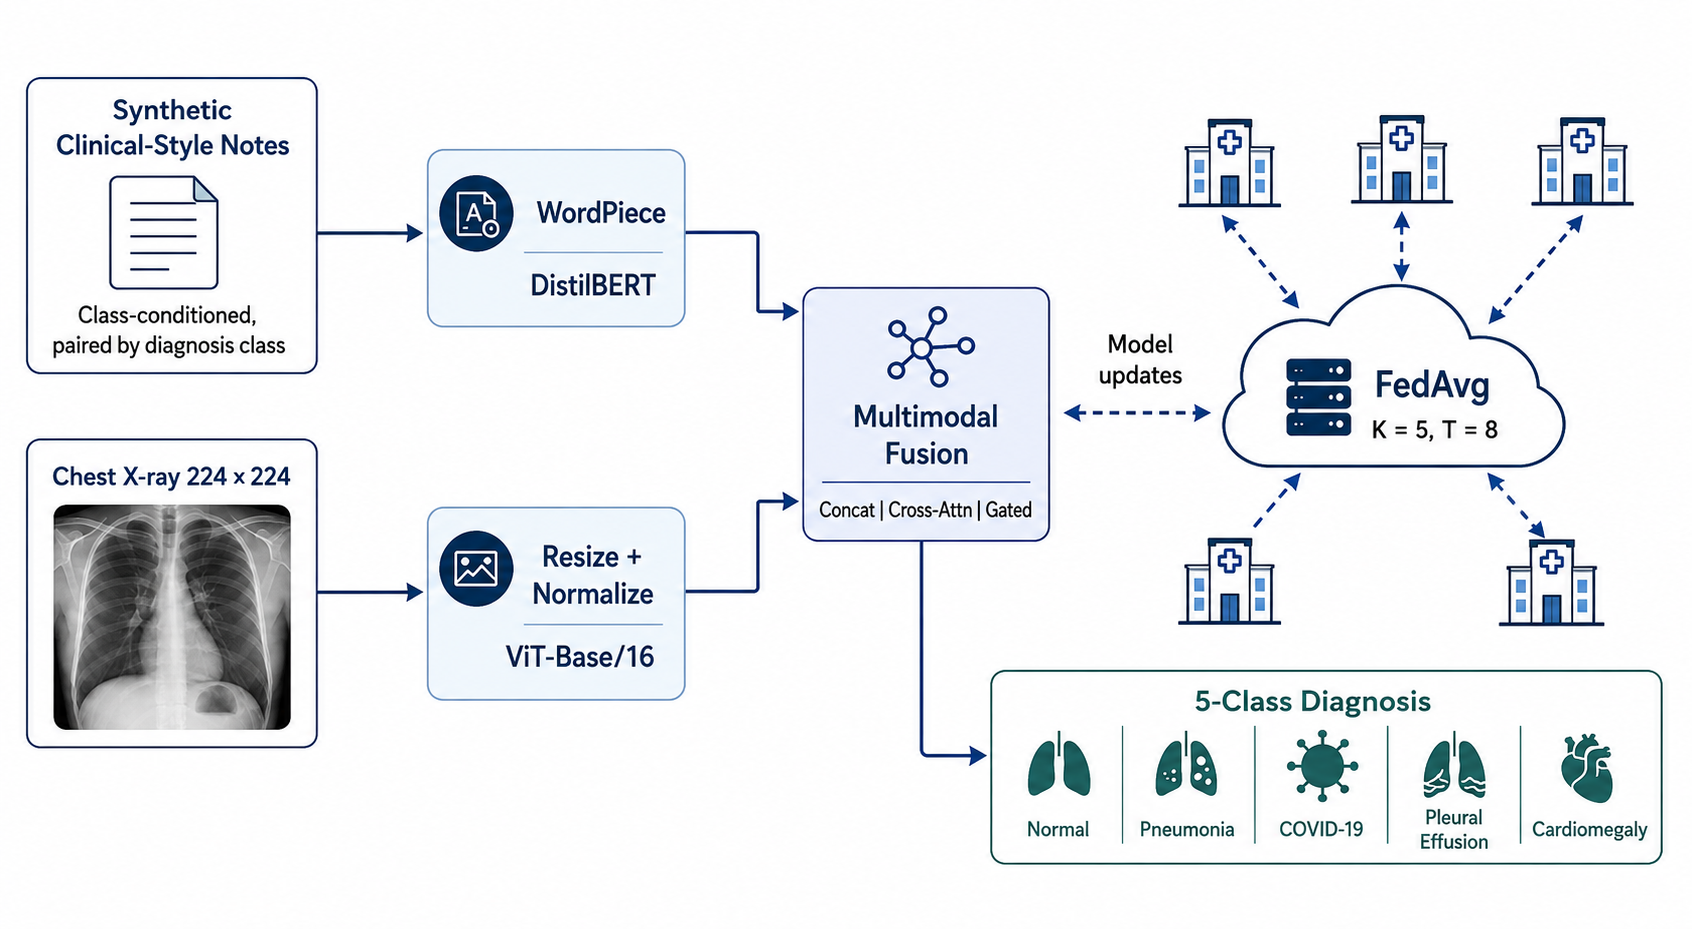
\includegraphics[width=\linewidth]
                         {generated/fig1b_omnimed_academic_architecture.png}};
  % Coordinates below are fractions of the bitmap: (0,0) lower left, (1,1) upper
  % right. The boundary encloses everything computed at one hospital and is
  % notched around the FedAvg cloud and the peer clients it serves.
  \begin{scope}[x={(pa.south east)}, y={(pa.north west)}]
    \draw[dashed, semithick, rounded corners=2pt, draw=fignavy]
      (0.008,0.968) -- (0.625,0.968) -- (0.625,0.303) -- (0.992,0.303) --
      (0.992,0.045) -- (0.008,0.045) -- cycle;
    \coordinate (pabadge) at (0.075,0.968);
    % "Server" in the free upper lobe of the FedAvg cloud, matched to the
    % bitmap's own sans-serif navy lettering.
    \node[inner sep=0pt, text=fignavy,
          font=\sffamily\bfseries\fontsize{5.5}{6}\selectfont]
          at (0.822,0.653) {Server};
  \end{scope}
  \node[anchor=west, fill=white, inner xsep=2pt, inner ysep=0.5pt,
        font=\scriptsize\bfseries, text=fignavy]
        at (pabadge) {Hospital Client $k$ (local computation)};
  \node[fill=white, inner sep=1pt, anchor=east] at (pabadge)
        {
\includegraphics[height=0.36cm]{generated/icon_hospital_client.png}};
\end{tikzpicture}
\par\vspace{1pt}\textbf{(a)}
\end{minipage}\hfill
\begin{minipage}[t]{0.40\textwidth}
\centering
\resizebox{0.98\linewidth}{!}{%
\begin{tikzpicture}[node distance=0.45cm]
  \node[llmbox] (ti)  {Text Input\\[-1pt]{\scriptsize Template clinical-style note}};
  \node[sbox, below=0.28cm of ti] (tok) {Tokenizer\\WordPiece};
  \node[llmbox, below=0.28cm of tok, text width=2.8cm, minimum height=1.0cm]
        (llm) {Text Encoder\\[-2pt]{\scriptsize DistilBERT}};
  \node[font=\scriptsize, below=0.18cm of llm] (ht)
        {$\mathbf{h}_t\!\in\!\mathbb{R}^{256}$};

  \node[vitbox, right=3.4cm of ti] (ii) {Image Input\\[-1pt]
                                         {\scriptsize Chest X-ray $224{\times}224$}};
  \node[sbox, below=0.28cm of ii] (aug) {Resize\\Normalize};
  \node[vitbox, below=0.28cm of aug, text width=2.8cm, minimum height=1.0cm]
        (vit) {Image Encoder\\[-2pt]{\scriptsize ViT-Base/16}};
  \node[font=\scriptsize, below=0.18cm of vit] (hv)
        {$\mathbf{h}_v\!\in\!\mathbb{R}^{512}$};

  \node[fedbox, right=2.1cm of vit, yshift=0.3cm, minimum height=1.4cm,
        text width=2.0cm] (fed)
        {Aggregation Server\\[-2pt]\textbf{FedAvg}\\[-1pt]
         {\scriptsize $K{=}3$--20 clients\\$T{=}8$ rounds}};

  \node[vlmbox, below=1.0cm of llm, xshift=3.1cm, minimum height=0.95cm]
        (vlm) {Multimodal Fusion\\[-2pt]
               {\scriptsize Concat $|$ Cross-Attn $|$ Gated $|$ Dual-Proj $|$
               Decoder A/B $|$ Cross-Attn-384 $|$ Token Encoder}};

  \node[mainbox=3.2cm, fill=vlmred!40, draw=vlmred,
        below=0.35cm of vlm] (cls)
        {Classification Head (5-class)\\[-1pt]
         {\scriptsize Focal + entropy/confidence penalties}};

  \node[outbox, below=0.35cm of cls] (out)
        {Normal $|$ Pneumonia $|$ COVID-19\\[-2pt]
         {\scriptsize Pleural Effusion $|$ Cardiomegaly}};

  \begin{scope}[on background layer]
    \node[draw=llmblue!80!black, fill=llmblue!4, rounded corners=6pt,
          dashed, thick, fit=(ti)(tok)(llm)(ht)(ii)(aug)(vit)(hv)(vlm)(cls)(out),
          inner sep=7pt] (client) {};
  \end{scope}
  \node[anchor=south west, fill=white, inner xsep=3pt, inner ysep=1pt,
        font=\scriptsize\bfseries, text=llmblue!80!black]
        (clientlbl) at ([xshift=1.05cm]client.north west)
        {Hospital Client $k$ (local computation)};
  \node[fill=white, inner sep=1pt, anchor=east] at ([xshift=-1pt]clientlbl.west)
        {
\includegraphics[height=0.70cm]{generated/icon_hospital_client.png}};

  \draw[arr](ti)--(tok);\draw[arr](tok)--(llm);\draw[arr](ii)--(aug);
  \draw[arr](aug)--(vit);\draw[arr](llm)--(ht);\draw[arr](vit)--(hv);
  \draw[arr](ht.south)--++(0,-0.15)-|(vlm.north west);
  \draw[darr](hv.south)--++(0,-0.15)-|(vlm.north east);
  \draw[arr](vlm)--(cls);\draw[arr](cls)--(out);
  \draw[<->, >=Stealth, thick, dashed]
        (client.east |- fed.center)--node[above, font=\tiny, align=center,
              inner sep=1.5pt]{model\\updates}(fed.west);
\end{tikzpicture}%
}
\par\vspace{1pt}\textbf{(b)}
\end{minipage}
\caption{OmniMed-FL architecture. (a) Overall multimodal federated workflow at the
reference $K{=}5$ setting; the dashed boundary encloses what runs inside a single
hospital client, and only model updates cross it to the FedAvg cloud shared by the
other clients. (b) Detailed architecture with the same client-side computation
boxed separately from the FedAvg aggregation server.}
\label{fig:arch}
\end{figure*}

\subsection{Federated Learning Setup}
\label{sec:objective}
Let $K$ clients hold disjoint shards $\mathcal{D}_k$ of the training split, with
$n_k=|\mathcal{D}_k|$ and $n=\sum_k n_k$, and let $\theta$ collect the trainable
parameters on the fusion path: both encoders, the projection layers, the fusion
operator, and the classification head. We minimize the sample-weighted empirical
risk
\begin{equation}
\begin{aligned}
\min_{\theta}\ F(\theta)&=\sum_{k=1}^{K}\frac{n_k}{n}F_k(\theta),\\[-2pt]
F_k(\theta)&=\frac{1}{n_k}\!\!\sum_{(x,z,y)\in\mathcal{D}_k}\!\!\ell\big(f_\theta(x,z),y\big).
\end{aligned}
\label{eq:fedobj}
\end{equation}
where $x$ is a radiograph, $z$ its class-paired note, $y$ the class label, and
$f_\theta$ the fused five-class classifier. Shards never leave a client, and the
server sees only the trainable tensors listed above. For mini-batch
$\mathcal{B}$, the loss we actually implement is
\begin{equation}
\ell_{\mathcal B}=\frac{1}{|\mathcal B|}\sum_{i\in\mathcal B}
(1-p_{i,y_i})^{\gamma}\mathrm{CE}_{\epsilon,i}
+\lambda\phi(h)+5[q-0.9]_+,
\label{eq:loss}
\end{equation}
with $p_{i,y_i}$ the true-class probability, $\mathrm{CE}_{\epsilon,i}$
label-smoothed cross-entropy, $\gamma{=}2$, $\epsilon{=}0.05$, $C{=}5$,
$h=H(\bar p)/\log C$, $q=|\mathcal B|^{-1}\sum_i\max_c p_{ic}$,
$\phi(h)=(1-h)[1-\tfrac{8}{3}[h-0.7]_+]$, and $[u]_+=\max(u,0)$.
The entropy-diversity term grows whenever a batch's predictions concentrate, and we
attenuate it above normalized entropy 0.7 so it stops pushing once the head is
healthy. Setting $\lambda{=}0$ removes that term alone, while the confidence
penalty $5[q-0.9]_+$ stays fixed everywhere. The class-balanced sampler and the
entropy-diversity term are the two anti-collapse components we ablate in
Section~\ref{sec:results}. Predicted-class diversity is the fraction of the five
labels that ever appear as a validation-set argmax.

Each round, the server broadcasts $\theta^{(t)}$, every eligible client runs three
local AdamW epochs on class-balanced mini-batches under eq.~\eqref{eq:loss}, clips the
gradient norm at one, and returns its trainable tensors for the sample-weighted
update in eq.~\eqref{eq:fedobj}. Operational runs start from public DistilBERT and
ViT-Base/16 weights with random task heads. We fine-tune both encoders and keep
unused unimodal heads and the inactive CNN fallback out of optimization and
communication.

\subsection{Controlled Proxy Corpus}

We built a balanced 3,000-image proxy corpus at 600 examples per class. Every
image is a public radiograph: sources include the Kermany pneumonia
collection~\cite{Kermany2018}, the NIH ChestX-ray dataset~\cite{Wang2017chestxray8},
and the COVID-19 Radiography Database~\cite{Chowdhury2020covid}. The controlled-v3
loader disables synthetic image generation and raises on any source shortfall;
its metadata records 3,000 public radiographs and no synthetic COVID-19 images.
Each class is drawn from a collection that labels it, which leaves the image axis
partly confounded with source collection. Images are resized to
$224{\times}224$, ImageNet-normalized, shuffled deterministically, and split 80/20
into 2,400 training and 600 validation examples.

\textbf{Clinical text data.}
We use no patient electronic health record (EHR) text, and the notes come from a
template engine. It pairs each image label, at
the class level, with a synthetic clinical-style note assembled from observation,
symptom, context, and indicator slots. To keep the network from memorizing an
obvious keyword we engineered the mix deliberately: 25\% of notes
draw every slot from the target class, 35\% mix target and non-target slots, and
40\% are heavily mixed while retaining a probabilistic target-class indicator.
This cuts direct label wording, but image and note do not come from the same
patient and must never be described as a real image--report pair.

\label{sec:corpus}
The corpus supports internal comparison, not absolute claims.
Every configuration (one choice of aggregation rule, fusion operator,
initialization, and anti-collapse components) trains and is scored on the same
corpus, so a gap between two of them is
attributable to the factor under test rather than to the data. Absolute scores carry
no such guarantee. Templates can leave
shortcuts, label-level pairing strips out the discordance and missingness of real
records, each class is drawn from a different source collection, and the split
is grouped by neither patient nor source.

\subsection{Experimental Setup}

\textbf{Hyperparameters.}
Table~\ref{tab:hyper} collects the protocol. Every client trains with AdamW
(learning rate $10^{-4}$, weight decay $0.01$) for three local epochs per round.
The suite runs eight rounds at batch size 16 in FP32, without automatic mixed
precision (AMP). Our reference setting is five clients at Dirichlet $\alpha=1.0$,
and Section~\ref{sec:results} varies $\alpha$ and the client count explicitly. Seeds
0 and 1 drive initialization, sampling, and partitioning, with one exception:
pooled-start reuses a single seed-0 checkpoint under seed-specific FL partitions. We
ran the frozen v3 suite in PyTorch 2.13.0+cu130 on one NVIDIA H100 NVL device;
the complete suite took 6.46 hours. The GPU-synchronized timer
wraps sequential local training and
aggregation within a round, and excludes validation, setup, I/O, networking,
concurrency, and multi-node throughput. Our timings are an execution-cost record,
not distributed throughput. We also did not force deterministic CUDA algorithms, so
a seed fixes the software pseudorandom streams without buying identical reruns.

\textbf{Partitioning.}
For each class, a Dirichlet draw allocates training indices across clients. Smaller
$\alpha$ concentrates client label distributions, and $\alpha\!\to\!\infty$
approaches independent and identically distributed (IID)
allocation~. A nominal $\alpha$ does not fully describe a finite split,
so we report the per-client class shares we actually drew alongside our scalability
results. The split is fixed across rounds for a given seed. Shards
holding fewer than four examples skip local optimization but still contribute the
unchanged global state at their sample weight. We do not renormalize over active
clients, which is why our cells report active alongside nominal $K$.

\textbf{Matched recent-method controls.}
Our FedMME-style baseline uploads each client model once and applies the one-shot
voting structure in~\cite{Wang2025fedmme}. Our implementation uses equal-weight hard
voting and breaks ties by mean softmax. We run it at two local
budgets. Our matched 24 epochs isolates the method from the budget; FedMME's native
100 epochs removes the budget discrepancy. Reporting both keeps the two confounds
separate. Either way it keeps the common corpus,
shard profile, encoders, and optimizer, substituting our five-class inputs for
FedMME's generated-report pipeline. The P-FIN-style stress test fixes
three multimodal and two image-only clients, projects both encoders to
256-dimensional normalized features, and compares zero filling, deterministic FIN,
Gaussian $\beta$-negative-log-likelihood ($\beta$-NLL) imputation ($\beta{=}0.5$),
and uncertainty-weighted aggregation with Fed-UQ-Avg balance weight 0.6 and
temperature 0.2~\cite{Shahid2026pfin}. We kept concatenation instead of P-FIN's
bidirectional cross-modal attention: with one pooled feature per modality,
cross-attention carries unit weight and collapses to a linear projection. FedProx
uses $\mu{=}0.01$. Each ablation changes one component and leaves every other
setting at the shared defaults that follow, most of which are fixed by what the
hardware allows. Three local epochs across eight rounds
give a tractable 24-local-epoch budget, and batch size 16 is what holds both encoders
plus one local model copy in GPU memory for the largest FP32 model. The grid crosses $K{=}\{3,5,10,20\}$ with $\alpha{=}\{0.1,1,5\}$ and the
$K{=}5$ sweep adds $\alpha{=}0.3$ and $0.5$, so the study spans severe to near-IID
skew; $K{=}5$ is our small cross-silo reference and $K{=}3$--20 probes count
sensitivity. Two seeds support descriptive claims, not significance. Everything else
in Table~\ref{tab:hyper} is a fixed default, not a per-model optimum.

\begin{table}[t]
\caption{Common simulation parameters.}
\label{tab:hyper}
\centering\footnotesize
\setlength{\tabcolsep}{4pt}
\begin{tabular}{llll}
\toprule
\textbf{Parameter} & \textbf{Value} & \textbf{Parameter} & \textbf{Value} \\
\midrule
Local Epochs ($E$)   & 3      & Seeds                    & 0, 1 \\
Fed.\ Rounds ($T$)   & 8      & Grid $K$ (ref.)          & 3, 5, 10, 20 (5) \\
Batch Size           & 16     & Grid $\alpha$ (ref.)     & 0.1, 1, 5 (1) \\
AdamW LR             & $10^{-4}$ & $K{=}5$ extra $\alpha$ & 0.3, 0.5 \\
Weight Decay         & $0.01$ & Precision                & FP32, no AMP \\
Diversity wt.\ ($\lambda$) & 1.0 & Init.                & Public enc.\ + rand.\ heads \\
\bottomrule
\end{tabular}
\end{table}

\section{Results}
\label{sec:results}

All quantitative results in this section come from the frozen
\texttt{controlled\_v3\_real5\_template\_text} run and its provenance-checked
merge. Scores are validation macro-F1. Error bars are sample standard
deviations over seeds 0 and 1 unless a single-run diagnostic is identified.

\subsection{Matched Baselines under Label Skew}

At $\alpha{=}0.1$ and $K{=}5$, local-only training averages 0.297 across the
five clients of one partition. Under the same corpus, partition, encoders,
optimizer, and 24-local-epoch budget, FedAvg reaches
$0.662\!\pm\!0.074$ and FedProx $0.737\!\pm\!0.085$
(Fig.~\ref{fig:baseline}). Their 0.075 gap lies inside the wider sample
standard deviation, so two seeds do not separate them. At $\alpha{=}1$, the
same ordering is 0.523 local-only, $0.820\!\pm\!0.029$ FedAvg, and
$0.862\!\pm\!0.019$ FedProx. Thus, both iterative federated methods sit well
above isolated client training at both skews.

Our SCAFFOLD--AdamW adaptation reaches only $0.070\!\pm\!0.015$ at
$\alpha{=}0.1$ and $0.236\!\pm\!0.205$ at $\alpha{=}1$. Its oscillatory
trajectory points to an unstable AdamW control-variate adaptation; this row
must not be read as a faithful evaluation of classical SGD-based SCAFFOLD.
The FedMME-style one-shot ensemble reaches $0.647\!\pm\!0.080$ at the matched
24-epoch budget and $0.609\!\pm\!0.109$ at its native 100-epoch budget.
Increasing local computation does not repair one-shot aggregation under
severe skew.

\begin{figure}[!t]
\centering
\begin{minipage}[t]{0.465\columnwidth}\centering

\includegraphics[width=\linewidth]{reviewer_matched_results_pa}\\[-5pt]
{\scriptsize\textbf{(a)}}
\end{minipage}\hfill
\begin{minipage}[t]{0.465\columnwidth}\centering
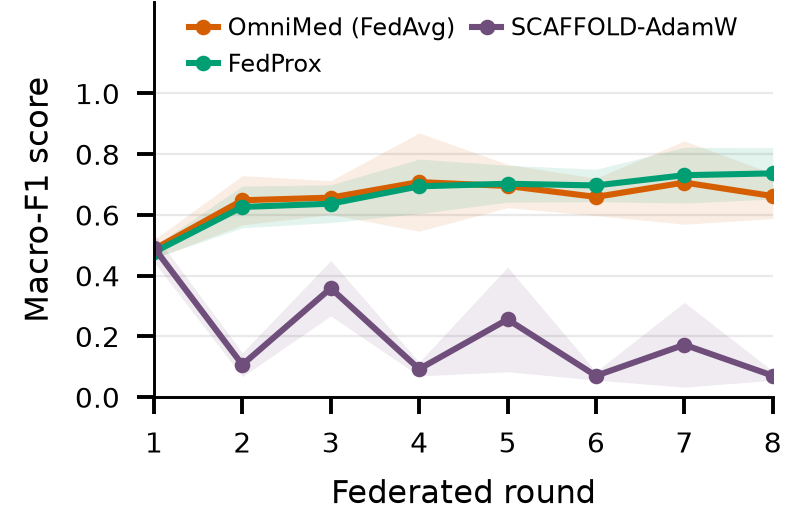
\includegraphics[width=\linewidth]{reviewer_matched_results_pb}\\[-5pt]
{\scriptsize\textbf{(b)}}
\end{minipage}
\caption{Controlled-v3 results at $\alpha{=}0.1$, $K{=}5$:
(a) matched baselines and (b) federated convergence.}
\label{fig:baseline}
\end{figure}

\subsection{Anti-Collapse, Fusion, and Initialization}

The anti-collapse ablation reverses the intended low-$\alpha$ ordering.
With the balanced sampler and entropy-diversity term, F1 is
$0.683\!\pm\!0.089$. Removing the sampler, the diversity term, or both raises
the mean monotonically to $0.716\!\pm\!0.055$,
$0.726\!\pm\!0.035$, and $0.758\!\pm\!0.016$
(Fig.~\ref{fig:anti_missing}(a)). Every one of the eight $\alpha{=}0.1$ runs
finishes at five-class diversity 1.0, including both unregularized seeds, so
final collapse is not observed. The full stack improves the mean minimum
diversity across rounds from 0.70 to 0.90, but it does so with a 0.075 F1
deficit to the unregularized configuration. At $\alpha{=}1$, all four
configurations maintain diversity 1.0 and score 0.809--0.846. We therefore
treat the stack as a transient coverage guard, not an accuracy-improving
component. Likewise, the non-federated early-abort controls score
$0.899\!\pm\!0.022$ with abort disabled and $0.871\!\pm\!0.012$ with it
enabled; neither branch collapses.

\begin{figure}[!t]
\centering
\begin{minipage}[t]{0.435\columnwidth}\centering
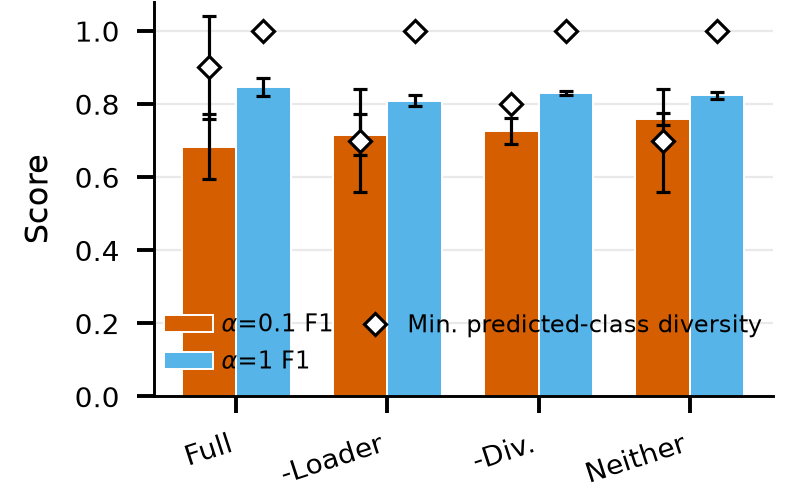
\includegraphics[width=\linewidth]{reviewer_matched_results_pc}\\[-5pt]
{\scriptsize\textbf{(a)}}
\end{minipage}\hfill
\begin{minipage}[t]{0.505\columnwidth}\centering
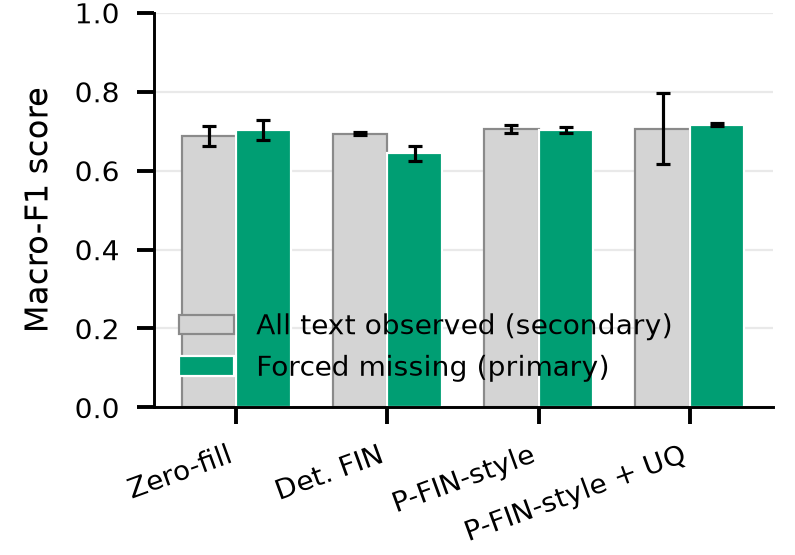
\includegraphics[width=\linewidth]{reviewer_matched_results_pf}\\[-5pt]
{\scriptsize\textbf{(b)}}
\end{minipage}
\caption{Controlled-v3 ablations: (a) anti-collapse F1 and minimum
predicted-class diversity; (b) forced-missing-text performance.}
\label{fig:anti_missing}
\end{figure}

The pooled-data fusion screen is a diagnostic architecture comparison, not an
operational FL result. Across two seeds, its eight operators span 0.750--0.925
F1. The 0.1755 spread is 33 times the 0.0053 median seed standard deviation,
so fusion choice carries real signal in this screen. Residual cross-attention
leads at $0.925\!\pm\!0.001$, while 384-dimensional cross-attention is last at
$0.750\!\pm\!0.002$; with only two seeds, the closely grouped leading methods
remain descriptively rather than statistically ordered. In the separate
operational sweep at $\alpha{=}0.1$, means span 0.636--0.759 but one operator's
sample standard deviation reaches 0.167, so that severe-skew sweep does not
resolve an operational winner (Fig.~\ref{fig:fusion_init}(a)).

The initialization control in Fig.~\ref{fig:fusion_init}(b) closes at
$0.647\!\pm\!0.022$ with all weights random and
$0.831\!\pm\!0.001$ with public encoders and random task heads. A pooled-data
checkpoint opens at 0.874 and closes at $0.877\!\pm\!0.007$, but it was
selected on the reporting split and is a non-deployable diagnostic oracle.
The operational public-encoder initialization retains 94.7\% of its final F1
without accessing pooled training data.

\begin{figure}[!t]
\centering
\begin{minipage}[t]{0.465\columnwidth}\centering

\includegraphics[width=\linewidth]{reviewer_matched_results_pd}\\[-5pt]
{\scriptsize\textbf{(a)}}
\end{minipage}\hfill
\begin{minipage}[t]{0.465\columnwidth}\centering

\includegraphics[width=\linewidth]{reviewer_matched_results_pe}\\[-5pt]
{\scriptsize\textbf{(b)}}
\end{minipage}
\caption{Controlled-v3 comparisons: (a) operational federated fusion under
severe skew; (b) federated initialization and non-federated abort controls.}
\label{fig:fusion_init}
\end{figure}

Under the forced-missing-text metric in Fig.~\ref{fig:anti_missing}(b), zero
filling, deterministic FIN, Gaussian $\beta$-NLL imputation, and
uncertainty-weighted aggregation score $0.688\!\pm\!0.025$,
$0.693\!\pm\!0.004$, $0.706\!\pm\!0.010$, and
$0.706\!\pm\!0.089$. The uncertainty-weighted rule ties the plain
probabilistic rule and is the noisiest, so this matched adaptation does not
show that uncertainty weighting tightens performance.

\subsection{Retrieval-Stage Evaluation}

Exact inner-product FAISS search~\cite{Johnson2021faiss} over training-fitted
TF--IDF note vectors gives condition-macro averages of 0.542 top-1 same-label
accuracy, 0.470 precision@5, and 0.706 mean top-1 cosine similarity across all
600 validation queries (Fig.~\ref{fig:retrieval}). Top-1 accuracy is above the
0.2 label prior but well below the similarity score, consistent with
synthetic templates whose neighbors can be lexically close without sharing a
label. This is a retrieval-stage diagnostic and establishes no clinical
generation quality.

\begin{figure}[!t]
\centering
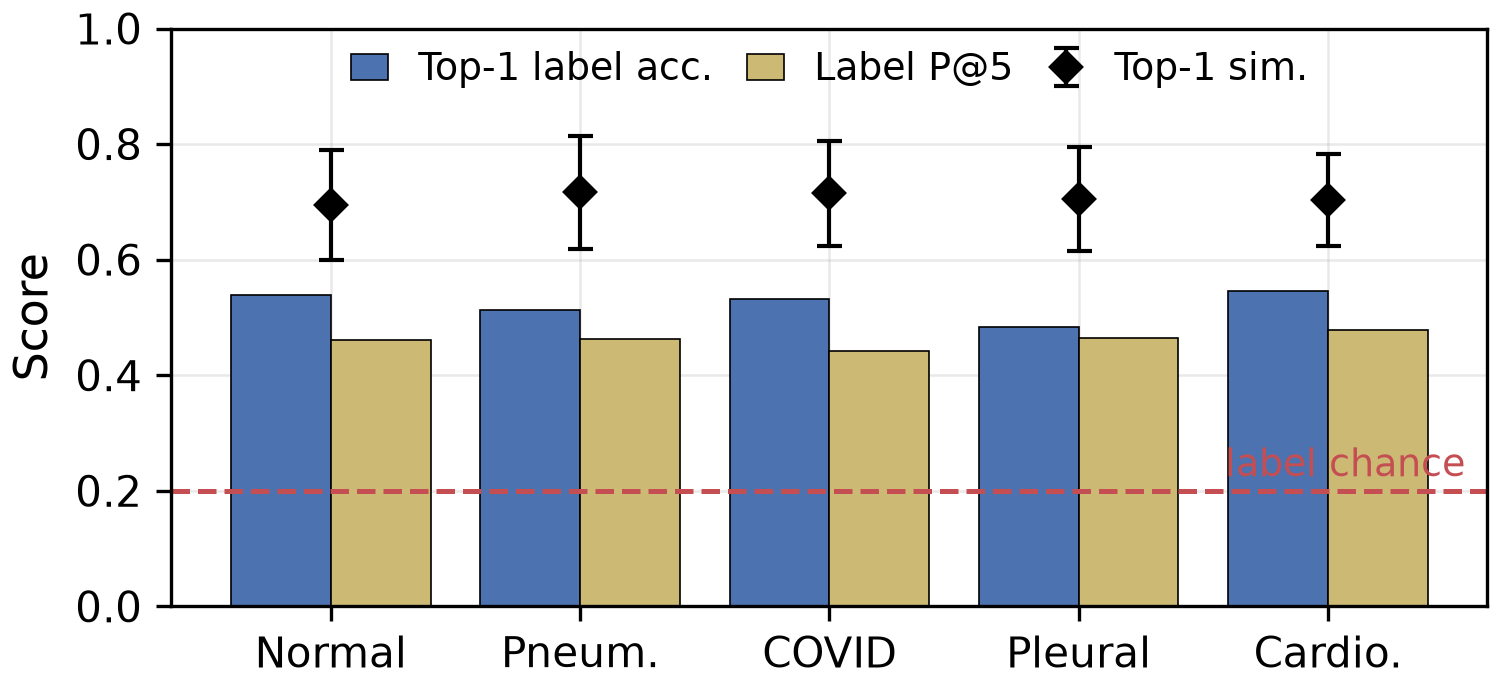
\includegraphics[width=0.72\columnwidth]{fig_rag_validated}
\caption{Controlled-v3 retrieval metrics by condition over 600 held-out
queries and a 2,400-note index.}
\label{fig:retrieval}
\end{figure}

\subsection{Scalability, Communication, and Resource Cost}

Figure~\ref{fig:scale_accuracy}(a) crosses
$K{=}\{3,5,10,20\}$ with $\alpha{=}\{0.1,1,5\}$. Every
$\alpha{=}5$ cell lies in 0.849--0.916 and every $\alpha{=}1$ cell in
0.818--0.862, whereas $\alpha{=}0.1$ yields 0.643--0.738 with spreads up to
$\pm0.159$. Within a row, increasing $K$ nearly sevenfold moves the mean by
at most 0.10 F1, while changing skew moves it by as much as 0.27. Client count
is therefore secondary to realized label allocation in this grid. Cells show
$A/K$, where $A$ counts shards with at least four samples; the severe
$K{=}20$ split has 17 active clients. Figure~\ref{fig:scale_accuracy}(b)
shows one realized partition in which individual clients hold nearly entire
classes.

\begin{figure}[!t]
\centering
\begin{minipage}[t]{0.465\columnwidth}\centering

\includegraphics[width=\linewidth]{reviewer_systems_scalability_pa}\\[-5pt]
{\scriptsize\textbf{(a)}}
\end{minipage}\hfill
\begin{minipage}[t]{0.465\columnwidth}\centering

\includegraphics[width=\linewidth]{reviewer_systems_scalability_pf}\\[-5pt]
{\scriptsize\textbf{(b)}}
\end{minipage}
\caption{Controlled-v3 scaling: (a) macro-F1 over client count and skew;
(b) one severe-skew client allocation.}
\label{fig:scale_accuracy}
\end{figure}

The GPU-synchronized sections in Fig.~\ref{fig:resources} take 41--62\,s per
round and allocate 4.77--5.92\,GiB on the shared H100. These panels are
execution records, not distributed-throughput curves: clients are simulated
sequentially, and uncontrolled server contention remains.

\begin{figure}[!b]
\centering
\begin{minipage}[t]{0.465\columnwidth}\centering

\includegraphics[width=\linewidth]{reviewer_systems_scalability_pb}\\[-5pt]
{\scriptsize\textbf{(a)}}
\end{minipage}\hfill
\begin{minipage}[t]{0.465\columnwidth}\centering
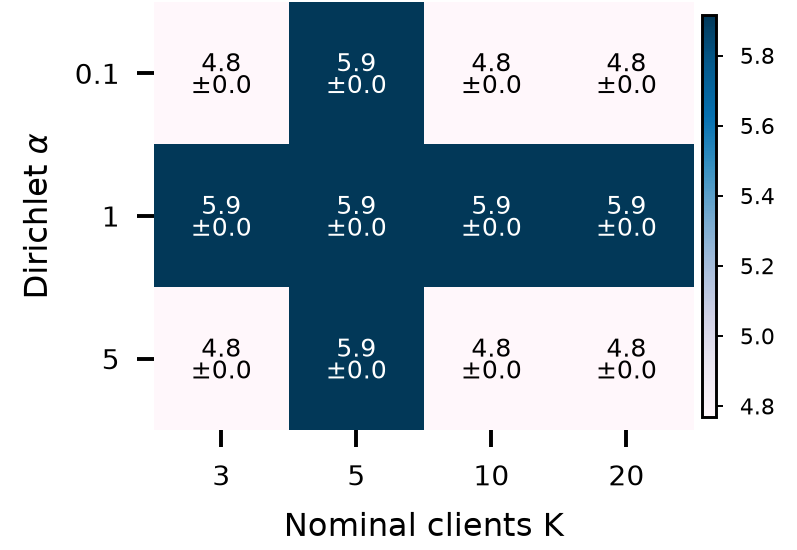
\includegraphics[width=\linewidth]{reviewer_systems_scalability_pc}\\[-5pt]
{\scriptsize\textbf{(b)}}
\end{minipage}
\caption{Controlled-v3 resource measurements: (a) seconds per round and
(b) peak allocated GPU memory.}
\label{fig:resources}
\end{figure}

For $|\theta|$ trainable parameters, $b$ bytes per parameter, $T$ rounds, and
nominal $K$, the plotted bidirectional volume is
\begin{equation}
V_{\mathrm{nom}}=2KT|\theta|b.
\label{eq:comm}
\end{equation}
Here $|\theta|{=}153{,}935{,}621$, $b{=}4$, and $T{=}8$, giving
27.5/45.9/91.8/183.5\,GiB at $K{=}3/5/10/20$. These are model-state
calculations, not measured network traffic; serialization, compression,
secure aggregation~\cite{Ergun2022globecom}, and algorithm-specific state are
excluded.

The matched single-seed branch audit at $\alpha{=}1$, $K{=}5$ scores text,
image, and concatenated multimodal models at 0.880, 0.768, and 0.830
(Fig.~\ref{fig:costs}(b)). Thus, concatenation improves on image-only by 0.062
but trails text-only by 0.050 in this run. Its one-way FP32 state is 0.573\,GiB
versus 0.248/0.324\,GiB, total timed rounds take 5.6 versus 1.8/4.3 minutes,
and peak allocation is 5.92 versus 2.84/4.33\,GiB. Fusion therefore incurs a
clear systems cost without guaranteeing a gain over the stronger unimodal
branch.

\begin{figure}[!b]
\centering
\begin{minipage}[t]{0.465\columnwidth}\centering
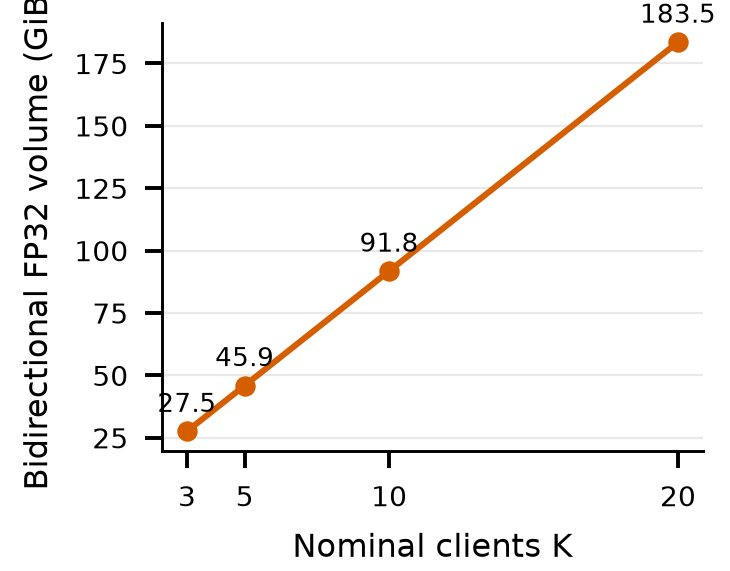
\includegraphics[width=\linewidth]{reviewer_systems_scalability_pd}\\[-5pt]
{\scriptsize\textbf{(a)}}
\end{minipage}\hfill
\begin{minipage}[t]{0.465\columnwidth}\centering

\includegraphics[width=\linewidth]{reviewer_systems_scalability_pe}\\[-5pt]
{\scriptsize\textbf{(b)}}
\end{minipage}
\caption{Controlled-v3 systems cost: (a) formula-derived FP32 model-state
volume; (b) single-seed modality score and measured resource audit.}
\label{fig:costs}
\end{figure}

\section{Discussion and Limitations}

The v3 rerun supports the paper's systems thesis but narrows two model claims.
Federation provides a large advantage over isolated local training, and
partition skew dominates client count. Fusion architecture also matters in
the pooled diagnostic screen. However, the operational concatenated model
does not beat text-only in the matched branch audit, and the anti-collapse
stack does not improve F1 under severe skew. We retain both negative findings
rather than overstate claims contradicted by v3.

The corpus remains a proxy: notes are synthetic and class-paired, not
patient-paired; template wording can leak class information; image class is
partly confounded with source collection; and the split is grouped by neither
patient nor source. Two seeds permit descriptive spreads, not significance,
and deterministic CUDA algorithms were not forced. Sequential single-GPU
simulation omits concurrency, latency, stragglers, dropout, and heterogeneous
hardware. Communication is analytic model-state volume rather than measured
network traffic. FedMME, P-FIN, and SCAFFOLD rows are declared adaptations,
not native replications. Consequently, none of the F1 or retrieval values
estimates clinical safety, generalization, or deployment readiness.

\newpage
\section{Conclusion}

On 3,000 public radiographs with class-paired synthetic notes, matched
controlled-v3 experiments show that FedAvg and FedProx outperform local-only
training at both tested skews, while label skew changes F1 more than a
near-sevenfold change in client count. Public encoders retain 94.7\% of a
pooled diagnostic oracle without pooled operational training. The fusion
screen shows genuine architecture sensitivity, but concatenation trails
text-only in the matched federated branch audit and costs $2.3\times$ its
model state. Removing both anti-collapse components improves severe-skew F1
from 0.683 to 0.758, with all runs finishing at full predicted-class
diversity. These findings define OmniMed-FL as a controlled systems benchmark
and motivate patient-paired, multi-institutional validation with more seeds,
native baseline implementations, and end-to-end network measurements.



\FloatBarrier
\bibliographystyle{IEEEtran}
\let\oldbibliography\thebibliography
\renewcommand{\thebibliography}[1]{%
  \oldbibliography{#1}%
  \fontsize{6.1}{6.6}\selectfont
  \setlength{\itemsep}{0.25pt}%
  \setlength{\parskip}{0pt}%
  \setlength{\parsep}{0pt}%
  \setlength{\topsep}{0pt}%
  \setlength{\labelsep}{3pt}%
  \linespread{0.98}\selectfont
}

\section*{Acknowledgment}
This work was supported in part by the Indian National Academy of Engineering
(INAE) Chair Professorship grant awarded to the third author.

\balance
\begin{thebibliography}{99}

\bibitem{Irvin2019}
J.~Irvin, P.~Rajpurkar, M.~Ko, \emph{et al.}, ``CheXpert: A large chest radiograph dataset with uncertainty labels and expert comparison,'' in \emph{Proceedings of the AAAI Conference on Artificial Intelligence}, volume~33, 2019, pages~590--597.

\bibitem{McMahan2017}
H.~B. McMahan, E.~Moore, D.~Ramage, S.~Hampson, and B.~Ag{\"u}era y~Arcas, ``Communication-efficient learning of deep networks from decentralized data,'' in \emph{Proceedings of the International Conference on Artificial Intelligence and Statistics}, volume~54, 2017, pages~1273--1282.

\bibitem{Sheller2020}
M.~J. Sheller, B.~Edwards, G.~A. Reina, \emph{et al.}, ``Federated learning in medicine: Facilitating multi-institutional collaborations without sharing patient data,'' \emph{Scientific Reports}, volume~10, article~12598, 2020.

\bibitem{Dou2021}
Q.~Dou, T.~Y. So, M.~Jiang, \emph{et al.}, ``Federated deep learning for detecting COVID-19 lung abnormalities in CT: A privacy-preserving multinational validation study,'' \emph{npj Digital Medicine}, volume~4, article~60, 2021.

\bibitem{Rajpurkar2017chexnet}
P.~Rajpurkar, J.~Irvin, K.~Zhu, \emph{et al.}, ``CheXNet: Radiologist-level pneumonia detection on chest X-rays with deep learning,'' \emph{arXiv:1711.05225}, 2017.

\bibitem{Dosovitskiy2021}
A.~Dosovitskiy, L.~Beyer, A.~Kolesnikov, \emph{et al.}, ``An image is worth 16$\times$16 words: Transformers for image recognition at scale,'' in \emph{Proceedings of the International Conference on Learning Representations}, 2021.

\bibitem{Lin2025fedlppa}
L.~Lin, Y.~Liu, J.~Wu, \emph{et al.}, ``FedLPPA: Learning personalized prompt and aggregation for federated weakly-supervised medical image segmentation,'' \emph{IEEE Transactions on Medical Imaging}, volume~44, number~3, pages~1127--1139, 2025.

\bibitem{Chu2022globecom}
D.~Chu, W.~Jaafar, and H.~Yanikomeroglu, ``On the design of communication-efficient federated learning for health monitoring,'' in \emph{Proceedings of the IEEE Global Communications Conference (GLOBECOM)}, 2022, pages~1128--1133.

\bibitem{Li2020fedprox}
T.~Li, A.~K. Sahu, M.~Zaheer, \emph{et al.}, ``Federated optimization in heterogeneous networks,'' in \emph{Proceedings of Machine Learning and Systems}, volume~2, 2020, pages~429--450.

\bibitem{Karimireddy2020}
S.~P. Karimireddy, S.~Kale, M.~Mohri, \emph{et al.}, ``SCAFFOLD: Stochastic controlled averaging for federated learning,'' in \emph{Proceedings of the International Conference on Machine Learning}, volume~119, 2020, pages~5132--5143.

\bibitem{Tian2022globecom}
Y.~Tian, Z.~Zhang, Z.~Yang, and R.~Jin, ``Hierarchical federated learning with adaptive clustering on non-IID data,'' in \emph{Proceedings of the IEEE Global Communications Conference (GLOBECOM)}, 2022, pages~627--632.

\bibitem{Zhang2025biomedclip}
S.~Zhang, Y.~Xu, N.~Usuyama, \emph{et al.}, ``A multimodal biomedical foundation model trained from fifteen million image--text pairs,'' \emph{NEJM AI}, volume~2, number~1, article~AIoa2400640, 2025.

\bibitem{Li2023llavamed}
C.~Li, C.~Wong, S.~Zhang, \emph{et al.}, ``LLaVA-Med: Training a large language-and-vision assistant for biomedicine in one day,'' in \emph{Proceedings of Advances in Neural Information Processing Systems}, volume~36, 2023, pages~28541--28564.

\bibitem{Wang2022medclip}
Z.~Wang, Z.~Wu, D.~Agarwal, and J.~Sun, ``MedCLIP: Contrastive learning from unpaired medical images and text,'' in \emph{Proceedings of the Conference on Empirical Methods in Natural Language Processing}, 2022, pages~3876--3887.

\bibitem{Wang2025fedmme}
N.~Wang, Y.~Deng, S.~Fan, \emph{et al.}, ``Multi-modal one-shot federated ensemble learning for medical data with vision large language model,'' \emph{arXiv:2501.03292}, 2025.

\bibitem{Shahid2026pfin}
N.~F. Shahid, M.~Ahmed, M.~A. Haider, \emph{et al.}, ``Probabilistic feature imputation and uncertainty-aware multimodal federated aggregation,'' in \emph{Proceedings of Medical Imaging with Deep Learning}, volume~315, 2026, pages~3593--3607.

\bibitem{Yan2024crossmodal}
Y.~Yan, H.~Wang, Y.~Huang, \emph{et al.}, ``Cross-modal vertical federated learning for MRI reconstruction,'' \emph{IEEE Journal of Biomedical and Health Informatics}, volume~28, number~11, pages~6384--6394, 2024.

\bibitem{Sanh2019}
V.~Sanh, L.~Debut, J.~Chaumond, and T.~Wolf, ``DistilBERT, a distilled version of BERT: Smaller, faster, cheaper and lighter,'' \emph{arXiv:1910.01108}, 2019.

\bibitem{Kermany2018}
D.~S. Kermany, M.~Goldbaum, W.~Cai, \emph{et al.}, ``Identifying medical diagnoses and treatable diseases by image-based deep learning,'' \emph{Cell}, volume~172, number~5, pages~1122--1131.e9, 2018.

\bibitem{Wang2017chestxray8}
X.~Wang, Y.~Peng, L.~Lu, \emph{et al.}, ``ChestX-ray8: Hospital-scale chest X-ray database and benchmarks on weakly-supervised classification and localization of common thorax diseases,'' in \emph{Proceedings of the IEEE Conference on Computer Vision and Pattern Recognition}, 2017, pages~2097--2106.

\bibitem{Chowdhury2020covid}
M.~E.~H. Chowdhury, T.~Rahman, A.~Khandakar, \emph{et al.}, ``Can AI help in screening viral and COVID-19 pneumonia?'' \emph{IEEE Access}, volume~8, pages~132665--132676, 2020.

\bibitem{Johnson2021faiss}
J.~Johnson, M.~Douze, and H.~J\'egou, ``Billion-scale similarity search with GPUs,'' \emph{IEEE Transactions on Big Data}, volume~7, number~3, pages~535--547, 2021.

\bibitem{Ergun2022globecom}
I.~Ergun, H.~U. Sami, and B.~G\"uler, ``Communication-efficient secure aggregation for federated learning,'' in \emph{Proceedings of the IEEE Global Communications Conference (GLOBECOM)}, 2022, pages~3881--3886.

\bibitem{Barros2022globecom}
P.~H. Barros and H.~S. Ramos, ``A novel aggregation method to promote safety security for poisoning attacks in federated learning,'' in \emph{Proceedings of the IEEE Global Communications Conference (GLOBECOM)}, 2022, pages~3869--3874.  \end{thebibliography}  \end{document}
